% !TEX root = ../macro.tex
\section{Solow Model}\label{sec:solow}

Growth accounting separates capital accumulation from productivity growth.
Solow adds a mechanism: some output becomes new capital, which changes future
production. We first ask why this mechanism was worth isolating, then derive
its dynamics and examine what it can explain.

\subsection{From the growth question to the model}\label{sec:solow-motivation}

\subsubsection{The problem behind the equations}

Investment has two roles. It uses current output and adds productive capacity.
For sustained growth, that capacity must remain compatible with the labor
available to operate it. The issue is not simply whether more investment raises
output, but whether saving and labor-force growth can generate a consistent
long-run path.

Solow's 1956 paper challenged the instability associated with the fixed
production proportions in the Harrod--Domar framework. His question was whether
that conclusion survived when firms could substitute capital for labor.
He retained a simple saving rule and studied adjustment under full employment.
This isolates a long-run mechanism; it does not establish that actual economies
always maintain full employment.\footnote{Robert M. Solow (1956), ``A
Contribution to the Theory of Economic Growth,'' \textit{Quarterly Journal of
Economics}, 70(1), 65--94, especially Sections I--III.
\url{https://doi.org/10.2307/1884513}. The presentation below uses modern
notation, gross output, and explicit depreciation.}

To see the issue in a simple fixed-proportions example, temporarily omit
technical change and write
\begin{equation}
Y=\min\left\{\frac{K}{v},\frac{L}{a}\right\},\qquad v,a>0.
\end{equation}
A unit of output requires $v$ units of capital and $a$ units of labor. If both
inputs are fully used, $K=vY$ and $L=aY$. A constant saving rate and depreciation
then imply
\begin{equation}
\frac{\dot K}{K}=s\frac{Y}{K}-\delta=\frac{s}{v}-\delta.
\end{equation}
But full use of both inputs also requires capital and output to grow at the
labor-force growth rate $n$. Thus
\begin{equation}\label{eq:solow-knife-edge}
\frac{s}{v}-\delta=n.
\end{equation}
The parameters need not satisfy this equality. If they do not, this fixed
production recipe cannot keep both inputs fully used along the proposed path.
This illustrates the compatibility problem, rather than all of Harrod's or
Domar's analysis.

Allow substitution and $K/Y$ is no longer fixed by a single recipe. More capital
per worker can raise output while reducing the extra output from another unit
of capital. This gives the capital-output ratio room to adjust. The question
becomes whether that adjustment brings investment into balance with the needs
of a growing labor force.

\subsubsection{Choosing what to keep}

The following is a way to build the model from that question, rather than a
reconstruction of the author's private sequence of ideas.
\begin{itemize}
\tightlist
\item \textbf{Keep a stock that carries the past forward.} Buildings, equipment,
and other productive assets are summarized by $K$. Gross investment adds to
this stock; depreciation removes part of it.
\item \textbf{Keep the inputs needed to use that stock.} Labor $L$ and its
efficiency $A$ enter production with capital. We initially take their paths as
given, so changes in capital do not also require a theory of fertility,
participation, or innovation.
\item \textbf{Close the flow of resources.} A single good can be consumed or
invested. With no government or foreign trade, saving becomes domestic
investment. A constant saving share closes this decision without solving a
household's intertemporal problem.
\item \textbf{Separate scale from intensity.} A large economy can have more
capital simply because it has more workers. Capital per effective worker
isolates whether productive assets are keeping up with labor and technology.
\end{itemize}
These choices produce a one-state accumulation model. Full employment removes
unemployment from the explanation; a common technology removes differences
across firms; the saving rule leaves preferences outside the model. Those
omissions make its mechanism visible and define its limits.

\subsection{Economic environment and assumptions}\label{economic-environment-and-specific-assumptions}

\subsubsection{Resources, timing, and behavior}

The economy is closed, has no government, and produces one good. Households own
capital and supply labor inelastically. Each worker supplies one unit of labor;
changes in hours, participation, and employment rates are omitted. Firms hire
labor and rent capital in competitive markets.

In discrete time, $K_t$ is available at the start of period $t$. Given $K_t$,
$A_t$, and $L_t$, firms produce $Y_t$. Households consume part of output and
save the fraction $s\in(0,1)$. Investment becomes available next period:
\begin{align}
Y_t&=C_t+I_t,\qquad I_t=S_t=sY_t,\label{eq:solow-resources}\\
K_{t+1}&=(1-\delta)K_t+sY_t,\qquad 0\leq\delta\leq1.\label{eq:solow-capital}
\end{align}
The saving rule is imposed. Firms still maximize profits; the absence of a
household optimization problem does not imply that firms are non-optimizing.

Technology and labor follow
\begin{equation}\label{eq:solow-exogenous}
A_{t+1}=(1+g)A_t,\qquad L_{t+1}=(1+n)L_t,
\qquad g,n\geq0.
\end{equation}
Initial $K_0,A_0,L_0$ are positive. We assume $\delta+n+g>0$ to obtain a finite
positive steady state below. Technology is labor-augmenting: an increase in
$A$ makes a worker provide more effective labor. Its availability and growth
are given, rather than explained by research or adoption decisions.

\subsubsection{Production and normalization}

Let
\begin{equation}\label{eq:solow-production}
Y_t=F(K_t,A_tL_t).
\end{equation}
$F$ has constant returns in capital and effective labor:
\begin{equation}
F(\lambda K,\lambda AL)=\lambda F(K,AL),\qquad \lambda>0.
\end{equation}
Replicating all inputs replicates output. This rules out a fixed factor, such
as land, that becomes scarcer as the economy expands. It also rules out
aggregate increasing returns in these two inputs.

Divide by effective labor and define
\begin{equation}\label{eq:solow-normalization}
k_t\equiv\frac{K_t}{A_tL_t},\qquad
 y_t\equiv\frac{Y_t}{A_tL_t}=F(k_t,1)\equiv f(k_t),\qquad
 c_t\equiv\frac{C_t}{A_tL_t}=(1-s)f(k_t).
\end{equation}
Here lower-case variables are \emph{per effective worker}. Output per worker is
$Y_t/L_t=A_ty_t$, and capital per worker is $K_t/L_t=A_tk_t$. This differs from
the per-hour normalization used for level accounting in Chapter~\ref{sec:growth-facts}.
With $A_t=1$, the two capital normalizations coincide.

Assume $f(0)=0$ and, for $k>0$,
\begin{equation}
f'(k)>0,\qquad f''(k)<0,\qquad
\lim_{k\downarrow0}f'(k)=\infty,\qquad
\lim_{k\to\infty}f'(k)=0.
\end{equation}
The last two are the Inada conditions on \emph{marginal products}, not output
levels. With the other assumptions, they make capital sufficiently productive
near zero and insufficiently productive at very high intensity to guarantee
an interior crossing of investment and replacement needs. They are sufficient
benchmark restrictions, not empirical laws for every technology.

Our running example is Cobb--Douglas:
\begin{equation}\label{eq:solow-cd}
F(K,AL)=K^\alpha(AL)^{1-\alpha},\qquad f(k)=k^\alpha,
\qquad 0<\alpha<1.
\end{equation}
Diminishing returns here means adding machines to a fixed amount of effective
labor produces progressively smaller additions to output. It does not mean
that output falls when capital rises.

\subsubsection{Prices and market clearing}

At each date, let $q_t$ be the real rental price of capital and $w_t$ the wage
per worker. A price-taking firm solves
\begin{equation}
\max_{K,L}\;F(K,A_tL)-q_tK-w_tL.
\end{equation}
At an interior solution, denoting derivatives with respect to the two arguments
of $F$ by $F_1,F_2$,
\begin{equation}
q_t=F_1(K_t,A_tL_t),\qquad w_t=A_tF_2(K_t,A_tL_t).
\end{equation}
Constant returns and Euler's theorem for homogeneous functions give
\begin{equation}
Y_t=F_1K_t+F_2A_tL_t=q_tK_t+w_tL_t.
\end{equation}
Economic profits are zero after paying both factors, including capital owned
by households. This is a property of this competitive constant-returns
benchmark, not a claim that owners receive no capital income.

For Cobb--Douglas, $q_t=\alpha k_t^{\alpha-1}$ and
$w_t=(1-\alpha)A_tk_t^\alpha$. Capital deepening lowers the rental return and
raises the wage per effective worker. Prices support full use of the supplied
capital and labor. Goods-market clearing and the saving rule then determine
investment. Given the initial stocks and exogenous paths, the model is closed.

\begin{greenblock}
\textbf{The mechanism in one loop.}
Capital and effective labor determine output; the saving rule turns some output
into investment; investment and depreciation determine next period's capital.
Factor prices describe the returns along this path. The saving rate does not
respond to those returns until we change the household side of the model.
\end{greenblock}

\subsection{Solow model in discrete time}\label{solow-model-in-discrete-time}

\subsubsection{Deriving the law of motion}

Define $D\equiv(1+n)(1+g)$, the gross growth factor of effective labor. Divide
\eqref{eq:solow-capital} by $A_{t+1}L_{t+1}$:
\begin{align}
k_{t+1}
&=\frac{(1-\delta)K_t+sY_t}{A_{t+1}L_{t+1}},\\
&=\frac{(1-\delta)K_t/(A_tL_t)+sY_t/(A_tL_t)}{D},\\
&=\frac{(1-\delta)k_t+sf(k_t)}{D}\equiv\Phi(k_t).
\label{eq:solow-discrete-map}
\end{align}
The numerator adds surviving capital and investment per current effective
worker. The denominator spreads it across next period's effective labor. New
workers need equipment, and increasing labor efficiency requires more equipment
per worker to keep $k$ constant.

Subtract $k_t$ and define $d_D\equiv D-1+\delta$:
\begin{equation}\label{eq:solow-discrete-change}
k_{t+1}-k_t=\frac{sf(k_t)-d_Dk_t}{D},\qquad
 d_D=\delta+n+g+ng.
\end{equation}
Break-even investment $d_Dk_t$ keeps capital per effective worker unchanged.
The $ng$ term is part of the exact discrete-time expression; dropping it is a
small-rate approximation. Setting $g=0$ gives $d_D=\delta+n$; setting $g=n=0$
gives $d_D=\delta$.

\subsubsection{A steady state and the path toward it}

A positive normalized steady state satisfies
\begin{equation}\label{eq:solow-discrete-steady}
k^*=\Phi(k^*),\qquad sf(k^*)=d_Dk^*,\qquad
\frac{K}{Y}=\frac{k^*}{f(k^*)}=\frac{s}{d_D}.
\end{equation}
A stable capital-output ratio is a conclusion \emph{on this path}, not something
that follows from labor-augmenting notation alone.

For existence and uniqueness, divide the middle equation by $k^*>0$. Strict
concavity and $f(0)=0$ imply $f'(k)<f(k)/k$, so
\begin{equation}
\frac{d}{dk}\frac{f(k)}{k}=\frac{kf'(k)-f(k)}{k^2}<0.
\end{equation}
The Inada conditions imply $f(k)/k$ falls from infinity to zero. Hence
$sf(k)/k=d_D>0$ has exactly one positive solution. Zero is also an absorbing
boundary under $f(0)=0$; our convergence result starts from $k_0>0$.

Below $k^*$, saving exceeds break-even investment and $k$ rises. Above $k^*$,
saving is insufficient to maintain that intensity and $k$ falls. Moreover,
\begin{equation}
\Phi'(k)=\frac{1-\delta+sf'(k)}{D}>0.
\end{equation}
Since $\Phi$ is increasing and $\Phi(k^*)=k^*$, an initial $k<k^*$ maps below
$k^*$, while an initial $k>k^*$ maps above it. The sequence is therefore
monotone and bounded toward $k^*$, and continuity makes its limit a fixed point.
The unique positive fixed point is the limit for every $k_0>0$.

\begin{center}
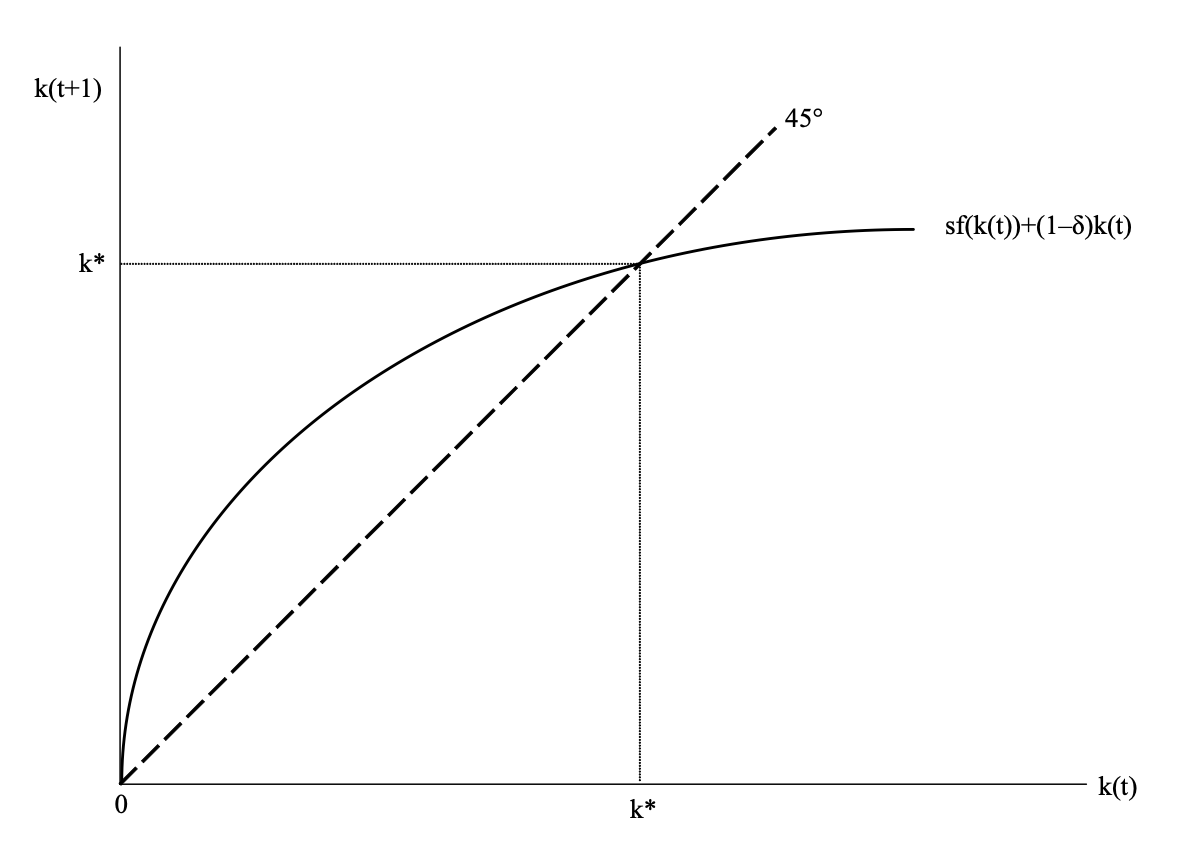
\includegraphics[width=0.85\linewidth]{images/solow_phase_diagram.png}
\end{center}
\noindent\textit{Reading the diagram.} This recovered diagram shows the special
case $n=g=0$, with $\delta>0$. The curved map is next period's capital; the
45-degree line is unchanged capital. Starting on the horizontal axis, move
vertically to the map, then horizontally to the 45-degree line to carry that
value into the next iteration. For $n>0$ or $g>0$, divide the map by $D$ as in
\eqref{eq:solow-discrete-map}.

A steady state is one particular equilibrium path. A transition from an
arbitrary initial stock is also an equilibrium path under the imposed saving
rule. Convergence does not make the transition cease to be an equilibrium.

\subsubsection{What grows on a balanced growth path?}

If $k_t=k^*$, then $y_t=f(k^*)$ and $c_t=(1-s)f(k^*)$ are constant. Yet
\begin{equation}\label{eq:solow-bgp}
\frac{Y_t}{L_t}=A_tf(k^*),\qquad
\frac{K_t}{L_t}=A_tk^*,\qquad
Y_t=A_tL_tf(k^*).
\end{equation}
Output and capital per worker grow at gross rate $1+g$; their aggregates grow
at $D$. With no technical progress, there is no sustained growth per worker on
this path, even if the population and total output keep growing.

For Cobb--Douglas, solve $s(k^*)^\alpha=d_Dk^*$:
\begin{equation}\label{eq:solow-cd-steady}
k^*=\left(\frac{s}{d_D}\right)^{1/(1-\alpha)},\qquad
y^*=\left(\frac{s}{d_D}\right)^{\alpha/(1-\alpha)}.
\end{equation}
A higher saving rate raises the long-run level of output per effective worker.
Holding the technology path fixed, it does not change the long-run growth rate
of output per worker. Its steady-state level elasticity is
\begin{equation}
\frac{\partial\log y^*}{\partial\log s}=\frac{\alpha}{1-\alpha}.
\end{equation}
This comparison holds other determinants fixed. It is not a causal estimate
from a cross-country correlation between saving and income.

\subsubsection{Saving, rebuilding, and conditional convergence}

Suppose an economy starts on its old balanced growth path and permanently
raises $s$. At the time of the change, $K$, $A$, and $L$ are inherited, so output
is unchanged and consumption falls. Higher investment raises future $K$; output
per worker then grows faster during the transition. As diminishing returns
reduce the extra investment generated by another unit of capital, $k$ approaches
its new, higher steady state. Long-run growth per worker returns to $g$.

This explains why an investment expansion can have a lasting level effect
without a lasting growth-rate effect. It does not establish that any observed
investment campaign will be productive: the one-good benchmark abstracts from
project selection, idle capacity, financing, and heterogeneous returns.

A one-time loss of physical capital, with technology, labor, and saving behavior
unchanged, lowers $k$. The high marginal product at the lower stock supports
rebuilding toward the same path. Actual disasters can also destroy skills,
institutions, and technology, so this experiment isolates a capital-loss
mechanism rather than predicting every recovery.

The convergence result is conditional on the determinants of $k^*$ and the
technology path. A low-income economy with a low saving rate or low productivity
need not grow faster than a richer economy already close to a higher path.
Income alone does not tell us distance from the relevant steady state.

\subsubsection{Local convergence speed}

Let $x_t=k_t-k^*$. A first-order Taylor expansion at $k^*$ gives
\begin{align}
k_{t+1}&=\Phi(k^*)+\Phi'(k^*)x_t+O(x_t^2),\\
x_{t+1}&\approx\phi x_t,\qquad
\phi\equiv\frac{1-\delta+sf'(k^*)}{D}.
\end{align}
Because $sf'(k^*)<sf(k^*)/k^*=d_D$, we have $0<\phi<1$. Iterating the
linearized system yields
\begin{equation}\label{eq:solow-discrete-speed}
x_t\approx\phi^t x_0,\qquad
\lambda_D=-\log\phi>0,\qquad
T_{1/2}\approx\frac{\log2}{\lambda_D}.
\end{equation}
$\phi$ is persistence; a larger $\phi$ means slower adjustment. $\lambda_D$ is
the corresponding decay rate per period, and $T_{1/2}$ is the local half-life
of a deviation. The original nonlinear path need not have this half-life far
from its steady state.

For Cobb--Douglas, $sf'(k^*)=\alpha d_D$, so
\begin{equation}
\phi=1-\frac{(1-\alpha)d_D}{D}.
\end{equation}
Adjustment is gradual because productive capacity is a stock. Investment can
change immediately, but only accumulated investment changes that stock.

\subsection{Solow model in continuous time}\label{solow-model-in-continuous-time}

\subsubsection{The same mechanism with continuous adjustment}

Now use continuous rates $\dot L/L=n$, $\dot A/A=g$, and depreciation rate
$\delta\geq0$, with $b\equiv n+g+\delta>0$. These are rates per unit of time;
they are not numerically identical to finite-period percentage changes. Write
\begin{equation}
\dot K=sF(K,AL)-\delta K,\qquad k=\frac{K}{AL},\qquad y=f(k).
\end{equation}
Log differentiation of the definition of $k$, followed by substitution, gives
\begin{align}
\frac{\dot k}{k}
&=\frac{\dot K}{K}-\frac{\dot A}{A}-\frac{\dot L}{L},\\
&=\frac{sY}{K}-\delta-g-n,\\
\dot k&=s\frac{Y}{AL}-(n+g+\delta)k
       =sf(k)-bk\equiv G(k).\label{eq:solow-continuous}
\end{align}
New investment increases capital intensity; depreciation, population growth,
and technical progress reduce it for a given aggregate stock. Technical
progress still raises productive possibilities: it reduces $k$ here because
each worker now represents more effective labor.

For a short time interval $\Delta t$, effective labor grows by approximately
$1+(n+g)\Delta t$ and depreciation is approximately $\delta\Delta t$. Applying
the discrete accounting over that interval gives
\begin{equation}
k(t+\Delta t)-k(t)
=\left[sf(k(t))-bk(t)\right]\Delta t+o(\Delta t).
\end{equation}
Divide by $\Delta t$ and take its limit to obtain
\eqref{eq:solow-continuous}. This explains why the continuous break-even rate
is $b$, whereas the exact discrete expression contains the product $ng$.

The positive steady state satisfies $sf(k^*)=bk^*$; $G(k)>0$ below it and
$G(k)<0$ above it. On the balanced growth path, $Y/L$ and $K/L$ grow at $g$,
$Y$ and $K$ grow at $n+g$, and $K/Y=s/b$. Under competitive pricing the net
instantaneous real return is $r=f'(k)-\delta$.

\subsubsection{Local approximation and an exact Cobb--Douglas solution}

Linearizing the law of motion around its steady state gives
\begin{align}
\dot k&\approx G'(k^*)(k-k^*),\\
G'(k^*)&=sf'(k^*)-b<0,\\
k(t)-k^*&\approx[k(0)-k^*]e^{-\lambda_Ct},
\qquad \lambda_C\equiv b-sf'(k^*)>0.\label{eq:solow-continuous-speed}
\end{align}
The exponential expression solves the \emph{linearized} system. It is generally
only a local approximation to the original nonlinear equation. For
Cobb--Douglas, $\lambda_C=(1-\alpha)b$ and the local half-life is
$\log2/[(1-\alpha)b]$.

Cobb--Douglas also permits an exact solution using a different variable. Set
$z(t)=k(t)^{1-\alpha}$ and differentiate:
\begin{align}
\dot z
&=(1-\alpha)k^{-\alpha}\dot k,\\
&=(1-\alpha)k^{-\alpha}(sk^\alpha-bk)
 =(1-\alpha)(s-bz).
\end{align}
This is a linear equation in $z$, with steady state $z^*=s/b$. Its solution
and the implied capital path are
\begin{align}
z(t)&=\frac{s}{b}+\left[z(0)-\frac{s}{b}\right]
 e^{-(1-\alpha)bt},\\
k(t)&=\left\{\frac{s}{b}+\left[k(0)^{1-\alpha}-\frac{s}{b}\right]
 e^{-(1-\alpha)bt}\right\}^{1/(1-\alpha)}.\label{eq:solow-exact-path}
\end{align}
Capital approaches its steady state without arriving there at a finite date
unless it starts there. ``Time to convergence'' must therefore specify a
tolerance or a half-life, rather than an exact date of arrival.

\subsection{The Golden Rule and the cost of saving}\label{golden-rate}

More saving raises steady-state output, but output is not consumption. To
maintain a larger capital stock, the economy must devote more resources to
investment. The Golden Rule asks which balanced growth path provides the
largest consumption per effective worker, holding the technology and labor
paths fixed.

In continuous time, a stationary $k$ requires investment $bk$, so feasible
steady-state consumption is
\begin{equation}\label{eq:solow-gr-consumption}
c^*=f(k)-bk.
\end{equation}
Maximize this expression over $k$:
\begin{align}
\frac{dc^*}{dk}&=f'(k)-b,\\
f'(k_{\mathrm{GR}})&=b=n+g+\delta,\qquad
\frac{d^2c^*}{dk^2}=f''(k)<0.\label{eq:solow-gr}
\end{align}
One extra unit of capital adds $f'(k)$ to output but requires $b$ units of
investment per unit of time to maintain its intensity. At the Golden Rule,
these marginal amounts are equal. Equivalently, the net marginal return
$f'(k_{\mathrm{GR}})-\delta$ equals $n+g$.

The saving rate that supports this stock satisfies
\begin{equation}
s_{\mathrm{GR}}=\frac{bk_{\mathrm{GR}}}{f(k_{\mathrm{GR}})}.
\end{equation}
For Cobb--Douglas, substitute
$\alpha k_{\mathrm{GR}}^{\alpha-1}=b$:
\begin{equation}
k_{\mathrm{GR}}=\left(\frac{\alpha}{b}\right)^{1/(1-\alpha)},
\qquad s_{\mathrm{GR}}=\alpha.
\end{equation}
In discrete time the argument is the same with $d_D$ replacing $b$:
$c^*=f(k)-d_Dk$ and $f'(k_{\mathrm{GR}})=d_D$. The Cobb--Douglas saving share
is again $\alpha$ under this timing convention.

\begin{blueblock}
\textbf{A welfare boundary.}
The Golden Rule maximizes consumption \emph{across balanced growth paths}.
Solow has not specified a utility function, discounting, or how to value the
consumption losses during a transition. It therefore does not establish that
moving toward the Golden Rule maximizes intertemporal welfare.
\end{blueblock}

If the initial steady state lies below $k_{\mathrm{GR}}$, raising saving toward
$s_{\mathrm{GR}}$ increases eventual consumption but requires sacrificing
consumption while capital is built. If it lies above $k_{\mathrm{GR}}$, reducing
saving toward the Golden Rule can raise both current and eventual consumption.
Investment is then maintaining more capital than is useful for maximizing
steady-state consumption. A high investment share alone is therefore not a
welfare criterion. Ramsey will specify preferences and make the transition
trade-off part of the saving decision; OLG will examine dynamic efficiency in
an economy with different generations.

\subsection{Extensions}

Solow model with money
\begin{itemize}
  \item Purvis, Douglas D. “Introducing Useful Money into a Growth Model.” The Canadian Journal of Economics / Revue Canadienne d’Economique 4, no. 3 (1971)
\end{itemize}

Augmented Solow model

\begin{itemize}
  \item N. Gregory Mankiw, David Romer, David N. Weil, A Contribution to the Empirics of Economic Growth, The Quarterly Journal of Economics, Volume 107, Issue 2, May 1992, Pages 407–437
\end{itemize}

AK model (often treated as a tool to introduce endogeneous growth model)

\begin{itemize}
  \item Romer, Paul M. (1986). "Increasing Returns and Long-Run Growth". Journal of Political Economy. 94 (5): 1002–1037.
\end{itemize}

Malthus to Solow (unified growth theory)

\begin{itemize}
  \item Hansen, Gary, D., and Edward C. Prescott. 2002. "Malthus to Solow ." American Economic Review, 92 (4): 1205–1217.
\end{itemize}
